% --- SLIDE 3: STATE OF THE ART ---
\begin{frame}{State of the Art: Passive Prosthetic Feet Overview}
    \begin{columns}[T]
        \begin{column}{\textwidth}
            \centering
            \vspace{-2em}
            % Tre immagini affiancate — sostituisci i nomi file con le tue foto
            \begin{figure}
                \centering
                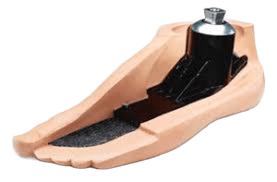
\includegraphics[width=0.21\linewidth]{image/sach.png}
                \hspace{3em}%\hfill
                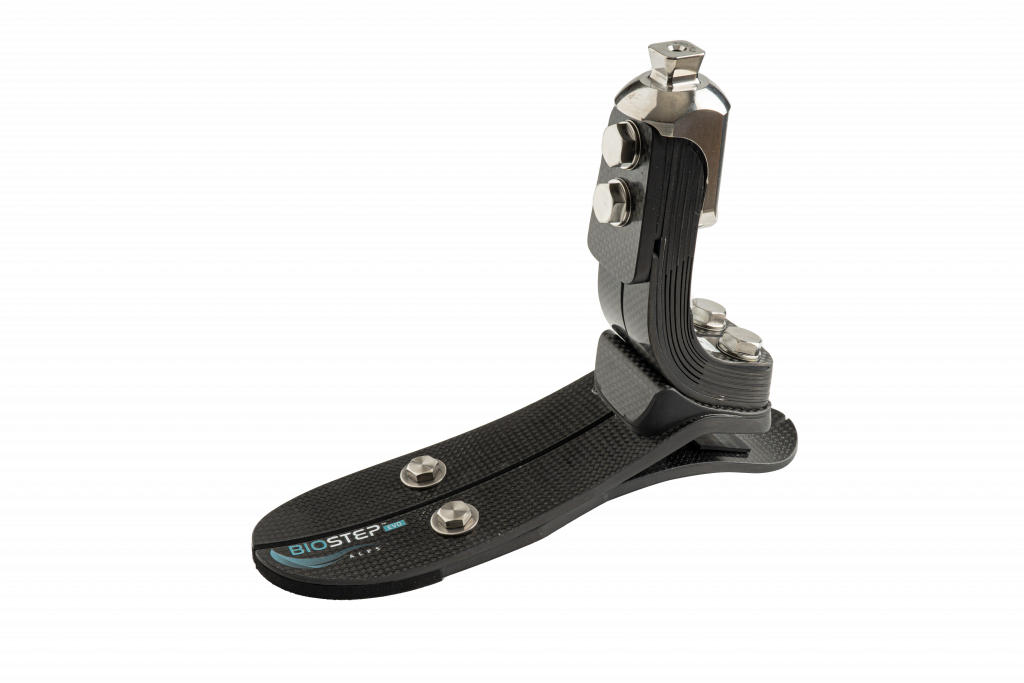
\includegraphics[width=0.21\linewidth]{image/esr_prostesis.png}
                \hspace{3em}%\hfill
                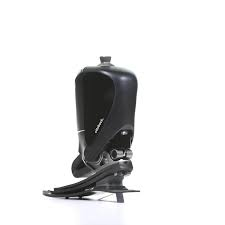
\includegraphics[width=0.21\linewidth]{image/ottobock.jpeg}
            \end{figure}

            \vspace{0.2cm}

            \begin{tabular}{p{4.5cm} p{4.5cm} p{4.5cm}}
                \toprule
                \textbf{SACH} & \textbf{ESR} & \textbf{Microprocessor (MPA)} \\
                \midrule
                \textbf{Pro:} Low cost, good initial shock absorption. & \textbf{Pro:} Elastic energy return, smooth roll-over (carbon fiber). & \textbf{Pro:} Real-time adaptation, reduces tripping risk. \\
                \textbf{Con:} No energy return, unnatural gait. & \textbf{Con:} Fixed stiffness. & \textbf{Con:} High cost, weight, recharging. \\
                \bottomrule
            \end{tabular}

        \end{column}
    \end{columns}
\end{frame}